\documentclass[a4paper,10pt]{article}
\usepackage[T1]{fontenc}
\usepackage[utf8x]{inputenc}
\usepackage{lmodern}
\usepackage{amssymb}
\usepackage{amsmath}
\usepackage{mathtools}
\usepackage[normalem]{ulem}
\usepackage{cancel}
\usepackage{enumitem}
\usepackage{graphicx}
%\usepackage[usenames,dvipsnames]{pstricks}
\usepackage{epsfig}
%\usepackage{pst-grad} % For gradients
%\usepackage{pst-plot} % For axes
\usepackage{tikz}
\newcommand*\circled[1]{\tikz[baseline=(char.base)]{
              \node[shape=circle,draw,inner sep=2pt] (char) {#1};}}
\title{Matte}
\author{Jakob Tigerström/Eric Johansson}

\begin{document}
\maketitle
\tableofcontents
\newpage
\begin{flushleft}
\section{TODO}
  \begin{enumerate}
    \item Skriv fler föreläsningar
    \item Kolla stavning
    \item Fixa warnings
    \item Skriv in föreläsnings ämne i section
    \item \sout{Överstryckning}
    \item Gör om bilder i geogebra eller liknande.
  \end{enumerate}
\section{Föreläsning 1}
  \subsection{Värdesiffror}
    Ex1: Hur många vädresiffror har talen
    \begin{enumerate}
      \item 251 3 st
      \item 0,251 3 st
      \item 0,001 1 st
      \item 250 2 eller 3 st\newline
      $ 2,5*10^2 $ 2 st\newline
      $ 2,50*10^2 $ 3 st
        \item 2500 2,3 eller 4 st
      $ 2,5*10^3 $\newline
      $ 2,50*10^3 $\newline
      $ 2,500*10^3 $
      \item 250,0 4 st
    \end{enumerate}
    Multiplikation och division: Svara med lika många värdesiffror som det värde som har minst värdesiffror.\newline
    5,22 *3.1 = 16,182 = 16.
  \subsection{Addition och Subtraktion}
    Minst antal decimaler avgör.\newline
    $ 23,52 + 12,4 = 35,92  \approx 35,9 $\newline
    $ 23,56 + 12,4 = 35,96  \approx 36,0 $
  \subsection{Uppskatta storleksordning}
    $ \frac{2,8*10^5}{3,2*10^3} $\newline
    Storleksordningen på svaret är $ 10^2 $
\section{Föreläsning 2}
  Omskrivning av formler\newline
  Densitet: $ \rho = m/v $\newline
  \subsection{Uppgifter}
    \subsubsection{EX1}
    Beräkna densiteten för en sten som har volymen $ 12cm^3 $ och väger $ 36 g $.\newline
    $ \rho = \frac{m}{v} = \frac{36}{12} = 3,0g/cm^3 $\newline \newline
  \subsubsection{EX2}
    Beräkna volymen av ett okänt föremål med densiteten $ 0,8g/cm^3 $ och väger $ 24g $.\newline
    $ \rho = \frac{m}{v} $\newline
    $ \rho * V \frac{m}{V} * V $\newline
    $ \frac{\rho * V}{\rho} = m $\newline
    $ V = \frac{m}{\rho} $\newline
    $ V=m/\rho = 24/0,8 = 30cm3 $ \newline
    Hooke lag\newline
    $ F=k*\Delta l $\newline
    F - kraft\newline
    k - fjäderkonstant\newline
    $ \Delta l $ - fjäderns förlägning\newline
  \subsubsection{EX3}
    Bestäm konstanten för en fjäder  som sträcks ut 18cm när den belastas med kraften 37N.\newline
    $ F=k*\Delta l $\newline
    $ \frac{F}{\Delta l} = k $\newline
    $ k = \frac{F}{\Delta l} = \frac{37}{0,18} = 205,55... \approx 2,1*10^2 N/m $\newline
    Formel för rörelse energi: $ w = \frac{mv^2}{2} $\newline
    w - energi(J)\newline
    m - massa(kg)\newline
    h - höjd(m)\newline
    g - gravitationskonstant.9,52m/s2\newline
    v - hastighet(m/s)\newline
  \subsubsection{EX4}
    Beräkna rörelseenergin för en bil som väger 1200kg och kör 90km/h\newline
    $ w = \frac{mv^2}{2} = \frac{1200*25^2}{2} = 375000 \approx 4*10^5 J = 400 kJ = 0,4 mJ $\newline
    $ 90km = 90000m $\newline
    $ 1h = 3600s $\newline
    $ \frac{90000}{3600} = \frac{90}{3,6} = 25m/s $\newline
  \newpage
  \section{Föreläsning 3}
    \subsection{Vektorer}
    Storhet som har både \underline{storlek} och \underline{riktning}.\newline
    Storheter där riktningen ej är relevant kallas \underline{skalärer}.\newline
    \textbf{Att skriva vektorer:}\newline
    \textbf{F}, (f)\newline
    \textbf{Att rita vektorer:}\newline
    $ \longrightarrow $\newline
    Pilens riktning är vektorens riktning.\newline
    Pilens längd är vektorens storlek.\newline
    \textbf{Att addera två vektorer:}\newline
    Parallellogrammetoden.\newline
    Polygonmetoden\newline
    Att multiplicera/dividera en vektor med en skalär(ett tal):\newline
    Multiplicera vektorn v(med tak) med talet $ k, k>0 $.\newline
    Sammar riktning ,storleken påverkas av $ k, k<0 $.\newline
    Motsatta riktningen storleken påverkas av k.\newline
    Komposanter(att dela upp en vektor)
    $ (x1;y1)+(x2;y2) = (x1+x2;y1+y2) $

  \section{Föreläsning 4}
    \subsection{Grundläggande algebra och prioriteringsregler}
    När vi beräknar värdet av ett uttryck måste vi ta hänsyn tilll prioriterings reglerna.
    \begin{enumerate}
      \item Paranteser
      \item Potenser
      \item Multiplikation och division
      \item Addition och division 
    \end{enumerate}
    \subsection{Uppgifter}
      \subsubsection{EX1}
        $ \underbrace{20/4}_{\text{3}}\underbrace{+8-}_{\text{4}}\underbrace{6*2}_{\text{3}}=\underbrace{5+8}_{\text{3}}\underbrace{-12}_{\text{3}}=1 $\newline
      \subsubsection{EX2}
        $ \underbrace{2*}_{\text{3}}\underbrace{5^3}_{\text{2}}=\underbrace{2*125}_{\text{3}}=250 $
      \subsubsection{EX3}
        $\underbrace{(8+5)}_{\text{1}}\underbrace{^2}_{\text{2}}\underbrace{(16+14)}_{\text{1}}=\underbrace{13^2}_{\text{2}}\underbrace{*30}_{\text{3}}=\underbrace{169*30}_{\text{3}}=5070 $

    Addition $ term+term=summa $\newline
    Subtraktion $ term-term=differens $\newline
    Multiplikation $ faktor*faktor=produkt $\newline
    Divistion $ \frac{täljare}{nämnare}=kvot $\newline
    \subsection{Bråkräkning}
    Multiplikation $ \frac{3}{5}*\frac{8}{7}=\frac{24}{35} $\newline
    Täljare multipliceras till en täljare.\newline
    nämnare multipliceras till en nämnare.\newline
    Addition och subtraktion.\newline
    $ \frac{1}{3}+\frac{1}{8}=\frac{8*1}{8*3}+\frac{1*3}{8*3}=\frac{8}{24}+\frac{3}{24}=\frac{11}{24} $

\section{Föreläsning 5 - uppställning och förenkling}
  %\subsection{Algebra - uppställning och förenkling}
  \subsection{Uppgifter}
    \subsubsection{EX1}
      Emil hyr en bil. Dygnsavgiften är 250kr och milkostnaden är 8kr/mil.\newline
      A) Hur mycket kostar det ifall Emil hyr bilen i ett dygn och kör 12 mil.\newline
      $ \underbrace{250}_{\text{Dygnsavg.}} + \underbrace{8*12}_{\text{mil kost.}} = 250+96 = 346kr $
      Svar: Det kostar honom 346kr \newline\newline
      B) Hur mycket ska Emil betala om han hyr bilen i k dygn och kör x mil?\newline\newline
      $ \underbrace{250k}_{\text{Dyngsavg.}} + \underbrace{8k}_{\text{mil kost.}}$ <- Algebraiskt uttryck\newline\newline


    \subsubsection{EX2}
      Annika lånar 15000kr för att köpa bil. Hon får betala 3\% i ränta.\newline
      A) Hur stor är hennes skuld efter 5år om hon ej har betalt tillbaka något.\newline
      $ \underbrace{15000}_{\text{Lån}} + \underbrace{1,03^5}_{\text{Förändringsfaktor}} \approx 17389kr $ \newline
      \textit{$^5 = antal år$} \newline
      Svar: Hon är skylldig ca 17389kr och är fast i lyxfällan \newline\newline
      B) Hur stor är skulden efter x år?\newline\newline
      $ \underbrace{15000}_{\text{Lån}} + \underbrace{1,03^x}_{\text{Förändringsfaktor}} $\newline\newline

    \subsubsection{EX3}
      Förenkla: $4x+3x+6-2$.\newline\newline
      $ \underbrace{4x+3x}_{\text{Addera}} + \underbrace{6-2}_{\text{subtrahera}} = 7x+4 $ \newline\newline

    \subsubsection{EX4}
      Förenkla: $\frac{5}{4}a-\frac{a}{2}$.\newline\newline
      $ \frac{5}{4}a-\underbrace{\frac{1}{2}a}_{\text{$\frac{a}{2}$}} = \frac{5}{4}a-\underbrace{\frac{1*2}{2*2}a}_{\text{Multiplicera}} = \frac{5}{4}a-\frac{2}{4}a = \frac{3}{4}a $\newline\newline

    \subsubsection{EX5}
      Förenkla: $a(a+b)-b(a-7b)$.\newline\newline
      $\underbrace{a(a+b)}_{\text{$a^2+ab$}} \underbrace{-}_{\text{-}} \underbrace{b(a+7b)}_{\text{$ab-7b^2$}} = a^2+ab-ab-7b^2 = a^2-7b^2 $\newline\newline

\section{Föreläsning 7}
  \subsection{Polynom}
    Ett polynom är en summa av termer där variablernas exponenter är possitiva heltal.\newline
    $ \underbrace{x^3+\overbrace{2}^{\text{Koeffcient}}x}_{\text{Variabel term}} - \underbrace{4}_{\text{Konstant term}} $
  \subsection{Multiplicera polynom}
    $ (a+b)(c+d) = ac+ad+bc+bd $\newline
    $ (a+b+)(c+d+e) = ac+ad+ae+bc+bd+be $\newline
  \subsection{Regler}
    \subsubsection{Konjugat regeln}
      $ \underbrace{(x+2)(x-2) }_{\text{Konjugat regeln}} = x^2-2x+2x-4 = x^2-4 $
    \subsubsection{Kvadrerings regelerna}
      $ \underbrace{(a+b)^2 = (a+b)(a+b) }_{\text{Kvadrerings regel}} = a^2+ab+ab+b^2 = a^2+2ab+b^2 $\newline
      $ \underbrace{(a-b)^2 = (a-b)(a-b)}_{\text{Kvadrerings regel}} = a^2-ab-ab+b^2 = a^2-2ab+b^2 $\newline
  \subsection{Uppgifter}
    \subsubsection{EX1}
      $ (a+5)(a-5) = a^2-5a+5a-25=a^2-25 $
    \subsubsection{EX2}
      $ (a+3)^2 = (a+3)(a+3) = a^2+6a+4 $
    \subsubsection{EX3}
      $ (3x+4y)^2 = 9x^2+2*3x*4y+16y^2 = 9x^2+24xy+16y^2 $
    \subsubsection{EX4}
      Faktorisera: $ 2xy^2+x^2y = xy(2y+x) $
    \subsubsection{EX5}
      Faktorisera: $ x^2-16 = (x+4)(x-4) $
    \subsubsection{EX6}
      Faktorisera: $ x^2+6x+9 = (x+3)^2 $
    \subsubsection{EX7}
      Faktorisera: $ 2x^2+10x+50 = 2(x^2+5x+25) $
    \subsubsection{EX8}
      Faktorisera: $ 5^x+5^{x+1} = 5^x+5^x*5 = 5^x(1+5 = 6*5^x $
    \subsubsection{EX9}
      Faktorisera: $ a^{2x+2}-a^{2x} = a^{2x}a^2-a^{2x} = a^{2x}(a^2-1) = a^{2x}(a+1)(a-1) $

\section{Föreläsning 11}
  \subsection{Logaritmer och logaritmlagar}
    "Logaritmen av 2000 är det tal vi måste upphöja 10 med för att få 2000".\newline\newline
    Definition: Om $ \underbrace{10^x = y}_{\text{potensform}} $ så är $ \underbrace{x=\log{y}}_{\text{logaritmform}} $\newline

    Hur löser vi 10$^x$=1000? Detta är lätt att lösa, antingen vet man att $x=3$ eller så testar man olika värden på x tills man kommer till något i närheten.
    Man kan även använda en grafritande räknare och kolla vart x skär 1000\newline
    Hur löser vi 10$^x$=2000? Detta är ett mycket svårare tal att lösa och görs lättast genom att använda logaritm, men man kan även använda en grafritande räknare.\newline

    $ \underbrace{10^x = 2000}_{\text{potensform}} $ -> $ \underbrace{x=\log{2000}}_{\text{logaritmform}} $\newline
    Svaret blir: $ x \approx 3,301 $

  \subsection{Logaritmlagarna}
    $ a = 10^{\log{a}}$ \newline
    Vi härleder logaritmlagarna med hjälp av potenslagarna
  \subsubsection{1:a lagen}
    AB = $10^{\log{A}}*10^{\log{B}} = 10^{\log{A}+\log{B}}$\newline
    AB = $ 10^{\log{AB}} $ \newline
    Lagen säger att "$\log{AB} = \log{A}+\log{B} $"
  \subsubsection{2:a lagen}
    $\frac{A}{B} = 10^{\log{A}}/10^{\log{B}} = 10^{(\log{A}-\log{B})}$\newline
    $\frac{A}{B} = 10^{\log{A/B}} $ \newline
    Lagen säger att "$\log{A/B} = \log{A}-\log{B} $"
  \subsubsection{3:e lagen}
    $A^k = \underbrace{A*A*A..*A}_{\text{k st}} = \underbrace{10^{\log{A}}*10^{\log{A}}*10^{\log{A}}..10^{\log{A}}}_{\text{k st}} = $\newline
    $= (10^{\log{A}})^k = 10^{k*\log{A}}$\newline\newline
    Lagen säger att "$\log(A^k) = k*\log{A} $"

  \subsection{Logoritm exempel}
    \subsubsection{EX1}
      Lös ekvationen $ 10^x = 67 $\newline\newline
      $ \underbrace{10^x = 67}_{\text{potensform}} $ -> $ \underbrace{x=\log{67}}_{\text{logaritmform}} $\newline
      Svaret blir: $ x \approx 1,8 $

    \subsubsection{EX2 - KONTROLLERA}
    Skriv talet 7 (exakt) som en potens med 10 som bas.\newline\newline
    Svar: $ 7 = 10^{\log{7}} $

  \subsubsection{EX3}
    Lös ekvationen $ 2*\log{x}=12 $\newline\newline
    $ 2*\log{x} = \underbrace{\frac{2*\log{x}}{2}}_{\text{Dividera med 2}} = \underbrace{\frac{12}{2}}_{\text{Dividera med 2}} = \log{x}=6 $ \newline\newline
    $ \log{x} = 6 $\newline
    $ x = 10^6 $\newline\newline
    Svar: $ x = 10^6$
  \subsubsection{EX4 - FIXA}
    Lös exakt $ 3^x = 8 $\newline\newline
    Alt1.\newline

    Alt2.\newline

    Svar: $ x = 1,9$

  \subsubsection{EX5}
    Lös: $\log{x} = \log{5}+\log{12}$\newline
    Lösning med 1:a lagen.\newline\newline
    $ \log{x} = \log{5}+\log{12} $\newline
    $ \log{x} = \underbrace{\log{5*12}}_{\text{Gör om log12 till 12}} $ \newline\newline
    $ \underbrace{\log{x}}_{\text{Ta bort log}} = \underbrace{\log{60}}_{\text{Ta bort log}}  $\newline\newline
    $ x = 60$\newline
    Svar: x = 60

  \subsubsection{EX6 - KONTROLLERA SVAR}
    Lös: $\log{x} = 2*\log{3}$\newline
    Lösning med 3:e lagen. \newline\newline
    $ \log{x} = 2*\log{3} $\newline
    $ \log{x} = \log{3^2} $ \newline\newline
    $ x = 3^2 $\newline\newline
    Svar: x = 60

  \subsubsection{EX7}
    Lös: $\log{x^2} = 8$\newline
    Lösning med 3:e lagen. \newline\newline
    $ 2*\log{x} = 8 $\newline\newline
    $ \underbrace{\frac{2*\log{x}}{2}}_{\text{Dividera med 2}} = \underbrace{\frac{8}{2}}_{\text{Dividera med 2}}  $ \newline\newline
    $ \log{x} = 4 $\newline\newline
    Svar: x = 4

\section{Föreläsning 12}
  \subsection{Uppgifter}
  \subsubsection{EX1}
    $ lgx = 2lg3+4lg2 $\newline
    $ lgx = lg(3^2)+lg(2^4) $\newline
    $ lgx = lg9+lg16 $\newline
    $ lgx = lg(9*16) $\newline
    $ x = 144 $
  \subsubsection{EX2}
    Lös ekvationen:\newline
    $ 2*3^x=4^x $\newline
    $ lg(2*3^x) = lg(4^x) $\newline
    $ lg2+lg(3^x) = xlg4 $\newline
    $ lg2+xlg3 = xlg4 $\newline
    $ lg2 = xlg4-xlg3 $\newline
    $ lg2 = x(lg4-lg3) $\newline
    $ x = \frac{lg2}{lg4-lg3} $
  \subsubsection{EX3 KONTOLLERA}
    Antag att vi vet att $ 10^{0,6}\approx4 $\newline
    Vad är då lg 400?\newline
    $ 10^{0,6}\approx4 $\newline
    $ 10^{0,6}*10^2\approx400 $\newline
    $ 10^{2,6}\approx400 $\newline
  \subsubsection{EX4}
    Lös ekvationen:\newline
    $ lg(x+4)+lg(x+2) = lg(x-1)+lg(x-10) $\newline
    $ lg((x+4)(x+2)) = lg((x-1)(x-10)) $\newline
    $ (x+4)(x+2) = (x-1)(x-10) $\newline
    $ x^2+2x+4x+8 = x^2-10x-x+10 $\newline
    $ \cancel{x^2}+6x+8 = \cancel{x^2}-11x+10 $\newline
    $ 6x+8 = -11x+10 $\newline
    $ 17x = 2 $\newline
    $ x = \frac{2}{17} $\newline
    $ lg(x-1) $ och $ lg(x-10) $ ej det, när $ x=\frac{2}{17} $ uppgiften saknar lösningar.
\subsubsection{EX5}
  Jordens folkmängd var år 2008 6,68 miljarder. Tillväxten var då $ 1,2\% $ per år.
  \begin{enumerate}
    \item Ställ upp en formel som ger jordens folkmängd om vi antar att den årliga procentuella ökningen ej ändras.\newline
    $ y=6,68*10^9*1,012^x $\newline
    x är anta år efter 2008. y är folkmängden x antal år efter 2008
    \item När är folkmängden 9 miljarder enligt denna modell?\newline
    $ 9*10^9 = 6,68*10^9*1,012^x $\newline
    $ 9*\cancel{10^9} = 6,68*\cancel{10^9}*1,012^x $\newline
    $ \frac{9}{6,68} = 1,012^x $\newline
    $ lg(\frac{9}{6,68}) = lg1,012^x $\newline
    $ lg(\frac{9}{6,68} = xlg1,012 $\newline
    $ x = \frac{lg(9/6,68)}{lg1,012} = 24,99 $\newline
    Svar: År 2033 är folkmängden på jorden 9 miljarder.
  \end{enumerate}
\subsubsection{EX6}
  I en kärnreaktor bildas bland annat plutonium-239 med en halveringstid på 24000 år.
  \begin{enumerate}
    \item Ställ upp och berätta hur mycket av 400 mg plutonium-239 finns kvar efter 100000 år.\newline
    $ 400*0,5^{x/24000} $\newline
    x är antalet år efter sönderfallets början. y är mängden plutonium-239 efter x är
    $ y = 400*0,5^{x/24000} $\newline
    $ y(100000) = 400*0,5^{100000/24000}\approx22mg $
    Svar: Det är 22 mg plutonium-239 kvar efter 100000 år.
    \item Hur länge måste man vänta om man vill att mängden plutonium ska gå ner till 1 promille av den ursprungliga mängden?\newline
    $ y = A*0,5^{x/24000} $\newline
    A är den ursprungliga mängden och x är antalet år sedan sönderfallets början, y är återstående mängd plutonium-239 vid tiden x år.
    $ \frac{A}{1000} = A*0,5^{x/24000} $\newline
    $ lg(\frac{1}{1000}) = lg(0,5^{x/24000}) $\newline
    $ lg(\frac{1}{1000}) = \frac{x}{24000}lg0,5 $\newline
    $ 24000lg(1/1000) = xlg0,5 $\newline
    $ x = \frac{24000lg(1/1000)}{lg0,5} = 240000år $\newline
    Svar: Det tar 240000 år innan mängden minskat till en promille.
  \end{enumerate}

\section{Föreläsning 13}
  \subsection{Likformighet}
    Alla kvadrater är likformiga\newline
    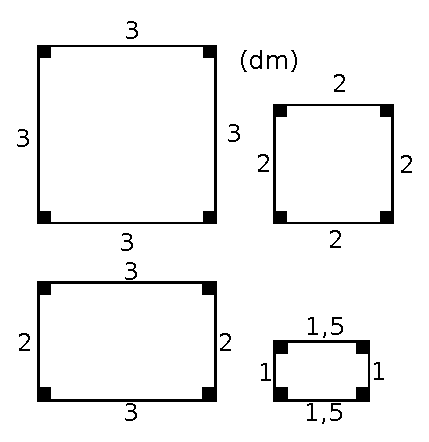
\includegraphics{likformighet.eps}\newline
    Dessa rektanglar är likformiga eftersom förhållandet mellan motsvarande sidor är lika.
    \subsubsection{Definition likformighet}
      Motsvarande vinklar är lika stora och förhållandet mellan motsvarande sidor är lika.

    \subsubsection{Likformiga trianglar}
      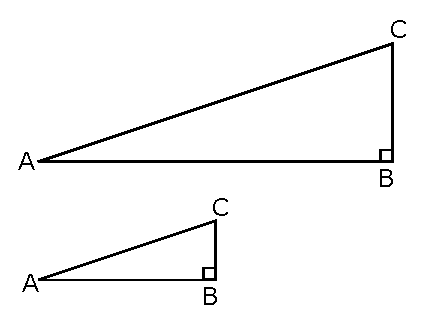
\includegraphics{likformighet2.eps}\newline
      Man behöver känna till två vinklar i varje triangel för att kunna jämföra dem och se om de är likformiga.
    \subsubsection{Likbelägnavinklar}
      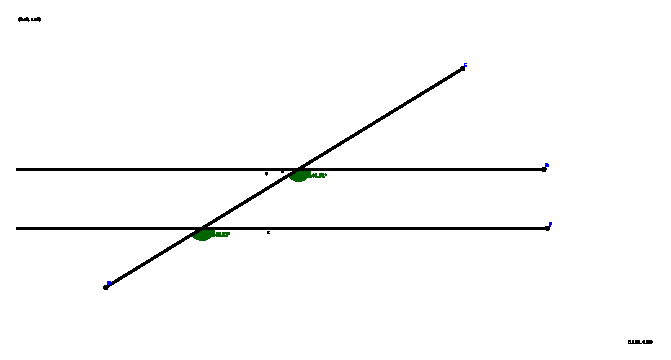
\includegraphics{likbelagna.eps}\newline
      Likbelägna vinklar är lika stora.
    \subsubsection{Transversalsatsen}
      $ \frac{b}{a} = \frac{d}{c} $
      $ \frac{a}{b} = \frac{c}{d} $\newline
  \subsection{Uppgifter}
    \subsubsection{EX1}
      Trianglarna är likformiga. Beräkna $x$ och $y$
      $ \frac{19,0}{12,0} = \frac{24,0}{y} = \frac{32,0}{x} $\newline
      $ y = \frac{19,0}{12,0} = 24,0 $\newline
      $ y = \frac{24,0*12,0}{19,0}\approx15,2cm $\newline
      $ \frac{19,0}{12,0} = \frac{32,0}{x} $\newline
      $ x = \frac{32,0*12,0}{19,0}\approx20,2cm $\newline
    \subsubsection{EX2}
      DE är paralell med AB. Bestäm $y$(sträckan CE)
      $ \frac{3,0}{5,0} = \frac{y}{6,0} $\newline
      $ y = \frac{3,0*6,0}{5,0} = 3,6cm$\newline
      Svar: $ y = 3,6cm $
\section{Föreläsning 14}
  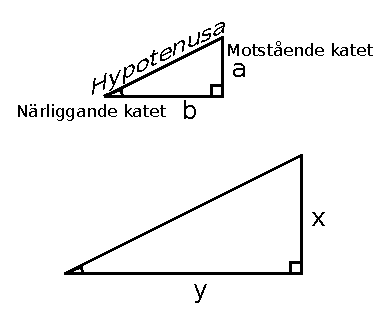
\includegraphics{trigonometri.eps}\newline
  $ \frac{a}{b} = \frac{x}{y} $\newline
  $ \frac{a}{b} = \frac{motstående katet}{närliggande katet} = \tan v $(uttalas "tangens" v)\newline
  Räknaren måste vara inställd på "degree" i mode.\newline
  \subsection{Uppgifter}
    \subsubsection{EX1}
      $ \frac{motstående katet}{närliggande katet} = \tan v $\newline
      $ motstående katet = \tan v * närliggande katet $\newline
      $ x = 15,0*\tan 38° $\newline
      $ x \approx 12 $\newline\newline
      Svar: Sidan x är 12cm.
    \subsubsection{EX2}
      Bestäm y\newline
      $ \tan 28° = \frac{z}{18} $\newline
      $ \tan 36° = \frac{y+z}{18} $\newline
      $ y+x 0 18 \tan 36° $\newline
      $ y = 18 \tan 36°-z = 18 \tan 36° - 18 \tan 28° \approx 3,5 $\newline\newline
      Svar: Sidan y är 3,5 cm.
    \subsubsection{EX3}
      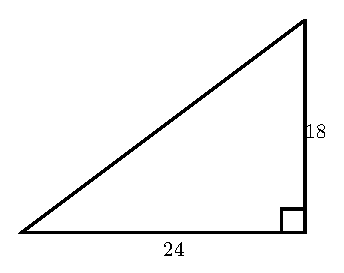
\includegraphics{trigonometri2.eps}\newline

      Skriv in från mobil bild.
    \subsubsection{EX4}
      Skriv in från mobil bild.
    \subsubsection{EX5}
      $ \sin 45° = \frac{a}{26} $\newline
      $ a = 26*\sin 45° $\newline
      $ \sin 35° = \frac{a}{x} $\newline
      $ x = \frac{a}{sin35°} = \frac{26\sin 45°}{\sin 35°} \approx 32cm $\newline
      Svar Sidan x är 32cm
    \subsubsection{EX6}
      Bestäm $ \sin u, \sin v, \cos u, \cos v $ . Ser vi något samband?\newline
      $ \sin u = \frac{12}{27} $\newline
      $ \sin v = \frac{\sqrt{585}}{27} $\newline
      $ \cos u = \frac{\sqrt{585}}{27} $\newline
      $ \cos v = \frac{12}{27} $\newline
      $ v+u = 90°$\newline$ v = 90°-u $\newline$ \sin u = \cos v = \cos(90°-u)$\newline$ \sin v = \cos u = \cos(90°-v) $
\section{Föreläsning 15}
  Medelvärde: Addera alla värden och dividera med antalet värden.\newline
  Medianvärde: Storleksordna alla värden, välj det mittersta värdet.\newline
  Typvärde: Det värde som förekommer flest gånger.\newline
  \subsection{Uppgifter}
    \subsubsection{EX1}
    \begin{enumerate}
      \item Dygnets maxtemperatur under en sommarvecka var $24,28,27,24,25,30,24$\newline
      Bestäm medelvärde , median och typvärde.\newline
      Medelvärde: $ \frac{24+28+27+24+25+30+24}{7} = \frac{182}{7} = 26 $\newline
      Median:  24,24,24,\circled{25},27,28,30  median = $25$\newline
      Typvärde: Förekommer 3 gånger.\newline
    \end{enumerate}

\end{flushleft}
\end{document}
